\documentclass[conference,a4paper,9pt]{IEEEtran}
\usepackage[spanish]{babel}
\usepackage[utf8]{inputenc}
\usepackage{multicol}
\usepackage{graphicx}
\usepackage{float}
\usepackage{cite}
\usepackage{amsmath}
\usepackage{subfig}
\usepackage{caption}
%\usepackage{balance}
\usepackage{url}

\hyphenation{}

\begin{document}
%\balance

\captionsetup[figure]{name=Fig.}
\title{Plataforma Robótica para Calibración de Sistemas Multi-Cámaras}

\author{
\IEEEauthorblockN{Martín Griffa, Leandro Yoaquino}
\IEEEauthorblockA{Universidad Tecnológica Nacional - Facultad Regional Córdoba\\
Sistemas de Comunicaciones III - Ing. Electrónica\\
\{martingriffacba, lyoaquino\}@gmail.com}}


\maketitle

\begin{abstract}
En el presente artículo se realiza el diseño e implementación de una plataforma robótica destinada a trabajar en aplicaciones que utilizan sistemas de múltiples cámaras. Estos sistemas, que han adquirido gran importancia en aplicaciones industriales y de investigación debido a su bajo costo y gran capacidad de recolección de datos, necesitan de un extenso proceso de calibración, que puede ser simplificado con el uso de una plataforma robótica. El robot diseñado cuenta con tracción diferencial de dos motores, controlados por un módulo driver comercial. Para la detección de obstáculos, la plataforma tiene 6 sensores infrarrojos medidores de distancia. El control en el dispositivo móvil se realiza con la placa de desarrollo KL46Z de Freescale, y hay una segunda unidad de control fija, encargada del procesamiento de datos y toma de decisiones. Para establecer una comunicación entre la unidad de control y la plataforma móvil, el robot cuenta con el módulo inalámbrico ESP8266 capaz de transmitir información vía Wi-Fi.
\end{abstract}

\IEEEpeerreviewmaketitle

\section{Introducción}

En aplicaciones de robótica, es común la necesidad de conocer la ubicación de un robot en un marco de referencia dado. Cuando se trabaja en ambientes exteriores la solución más utilizada es el GPS, pero se vuelve inviable en ambientes interiores. En estos casos, el recurso de la odometría por medio de encoders para obtener la ubicación absoluta es también problemática debido al error acumulado por los mismos \cite{encoders}. En otras aplicaciones, llamadas de tracking o seguimiento, es necesario determinar la ubicación de personas u objetos en el espacio, \cite{tracking}. Las cámaras son sensores relativamente económicos y precisos que solucionan los inconvenientes que presentan los métodos convencionales, lo que llevó a que adquieran gran importancia en este tipo de aplicaciones en el último tiempo  \cite{camara1}, \cite{camara2}, \cite{camara3}.

En un sistema de seguimiento o tracking el objetivo es determinar la posición de un objeto en un marco de referencia predeterminado. En el caso de ambientes de trabajo interiores los sensores más utilizados para realizar estas mediciones son las cámaras. Éstas tienen la desventaja de tener un rango de trabajo acotado debido a que existe una solución de compromiso entre el campo de visión y la resolución requerida por el problema. Debido a ello, normalmente la mejor solución consiste en el uso de múltiples cámaras, ubicadas adecuadamente, de tal manera que abarquen el mayor área posible sin detrimento de la resolución.

Un sistema de múltiples cámaras es un conjunto de sensores desplegados en un área determinada. El empleo de estos sistemas se ha extendido notablemente en los últimos años debido al bajo costo de los mismos y a su gran capacidad para generar información. Entre los usos más comunes podemos nombrar sistemas de seguridad, vigilancia, control de acceso, análisis de situaciones deportivas, monitorización del tráfico, navegación autónoma, entre otras \cite{camara2}, \cite{camara3}. También en el ámbito académico y de investigación, son usados en sistemas de seguimiento y guiado de vehículos autónomos y robots \cite{camara1}, \cite{diego}, \cite{kulich}.

En este artículo se plantea el desarrollo de una plataforma robótica que facilite el trabajo con sistemas de cámaras, partiendo de la base que sea económica, desarrollada con herramientas que estén a nuestra disposición y simple de programar. En la Sección \textit{II} se justifica la necesidad de la plataforma y se mencionan las posibles aplicaciones en las que puede utilizarse. Por otro lado, en la Sección \textit{III} se describe el diseño de la estructura del robot, los motores utilizados y los fundamentos teóricos relacionados con la velocidad lineal y angular del robot. En la Sección \textit{IV} se analiza y selecciona el módulo de comunicación inalámbrica, mientras que en la sección \textit{V} se detallan los distintos elementos que conforman el hardware de la plataforma. Además, en la Sección \textit{VI} se explican los programas que integran este proyecto, los cuales se encuentran divididos en una aplicación central de control basada en LabView y un programa en C cargado en el microcontrolador de la plataforma. Finalmente, en \textit{VII} se realiza un balance del diseño realizado y se proponen ciertas mejoras para optimizar el funcionamiento del plataforma.

\section{Motivación del proyecto}

Todos los sistemas de cámaras deben estar calibrados para permitir cualquier tipo de procesamiento de los datos obtenidos. Calibrar una cámara o un sistema de cámaras, implica caracterizar todos los elementos que componen el sistema, expresando matemáticamente las relaciones existentes entre ellos. A la hora de implementar esta calibración, uno de los métodos más utilizados consiste en realizar una serie de tomas con las cámaras, en las cuales se pueda observar un patrón o fiducial, de dimensiones y características conocidas. Luego, mediante distintos algoritmos, esas imágenes son procesadas, obteniéndose los parámetros de calibración del sistema. Para llevar a cabo este procedimiento es necesario contar con un banco de pruebas o plataforma de experimentación que traslade el patrón por los distintos planos de las cámaras, agilizando y optimizando la toma de imágenes necesarias. Considerando que para obtener una buena calibración, el patrón debe ser visto por la cámara desde distintos ángulos y distancias, y que además las cámaras deben permanecer estáticas en el marco de referencia global, es inevitable que el patrón deba moverse por el entorno durante el proceso de calibración.

Una plataforma sería la encargada de realizar esta tarea, pero la mayoría de las que se encuentran en el mercado son costosas y utilizan sistemas complejos en su programación. El objetivo planteado a la hora del diseño del proyecto fue desarrollar e implementar el control de una plataforma robótica que tuviera la capacidad de desplazarse sobre un área determinada, siguiendo las instrucciones que el usuario indique mediante un joystick. El dispositivo debe evitar las colisiones con los obstáculos que se encuentren en su trayectoria, valiéndose de la información provista por sensores infrarrojos.

Además de transportar el patrón utilizado para la calibración de sistemas de cámaras, una plataforma de estas características podría ser utilizada para testear algoritmos de tracking o seguimiento. Como la plataforma realiza una trayectoria controlada y predecible, los resultados obtenidos con el tracking pueden ser comparados con las órdenes de control del robot para calcular el error en la estimación de la posición y mejorar el funcionamiento del algoritmo.

\section{Mecánica del robot}

El movimiento del robot está basado en una tracción diferencial, la cual es una configuración muy común para sistemas utilizados en interiores, debido a que permite al robot girar sobre su propio eje. De esta manera, el dispositivo puede moverse en espacios congestionados con cierta facilidad. La tracción diferencial utiliza dos ruedas controladas individualmente con dos puntos fijos de apoyo. La plataforma cuenta con dos motores de corriente continua con caja reductora a $50\mathrm{rpm}$. El desplazamiento del robot a lo largo de la trayectoria está determinado por
\begin{equation}
D = \frac{D_l + D_r}{2},
\label{eq:desplazamiento}
\end{equation}
donde $D$ es el desplazamiento del robot, $D_l$ es el desplazamiento de la rueda izquierda y $D_r$, el de la rueda derecha.

De la misma forma, la velocidad lineal del robot se obtiene mediante
\begin{equation}
V = \frac{V_l + V_r}{2}.
\label{eq:velocidad}
\end{equation}
Análogamente a la expresión del desplazamiento, $V$ indica la velocidad del robot, y $V_l$ y $V_r$ indican las velocidades del motor izquierdo y derecho, respectivamente.

La ecuación
\begin{equation}
\theta = \frac{D_l - D_r}{d}
\label{eq:desplazamiento_angular}
\end{equation}
determina el desplazamiento angular del robot, que se calcula teniendo en cuenta la distancia de separación entre ruedas $d$, que es un dato de diseño.

El cambio de orientación del vehículo es función de los desplazamientos de las ruedas. Cabe mencionar que la variable $d$ en el denominador representa una fuente de error significativa debido a las incertidumbres asociadas con el punto de contacto efectivo. Estos errores se deben a los desplazamientos indeseados ocasionados por las irregularidades del piso. Adicionalmente, los diámetros de las ruedas pueden variar minúsculamente debido a que los anillos son de goma y por lo tanto son comprimidos por el peso. Todas estas fuentes de error hacen que el vehículo se desvíe de la trayectoria deseada.

El robot tiene un aspecto circular; el diámetro de la base de la plataforma es de $25\mathrm{cm}$ y junto con el módulo sensorial llega a tener una altura de $17\mathrm{cm}$. En la Fig. \ref{render} se puede observar un render del robot, donde se muestra la forma de las ruedas y la ubicación de los motores y sensores.

\begin{figure}%
\centering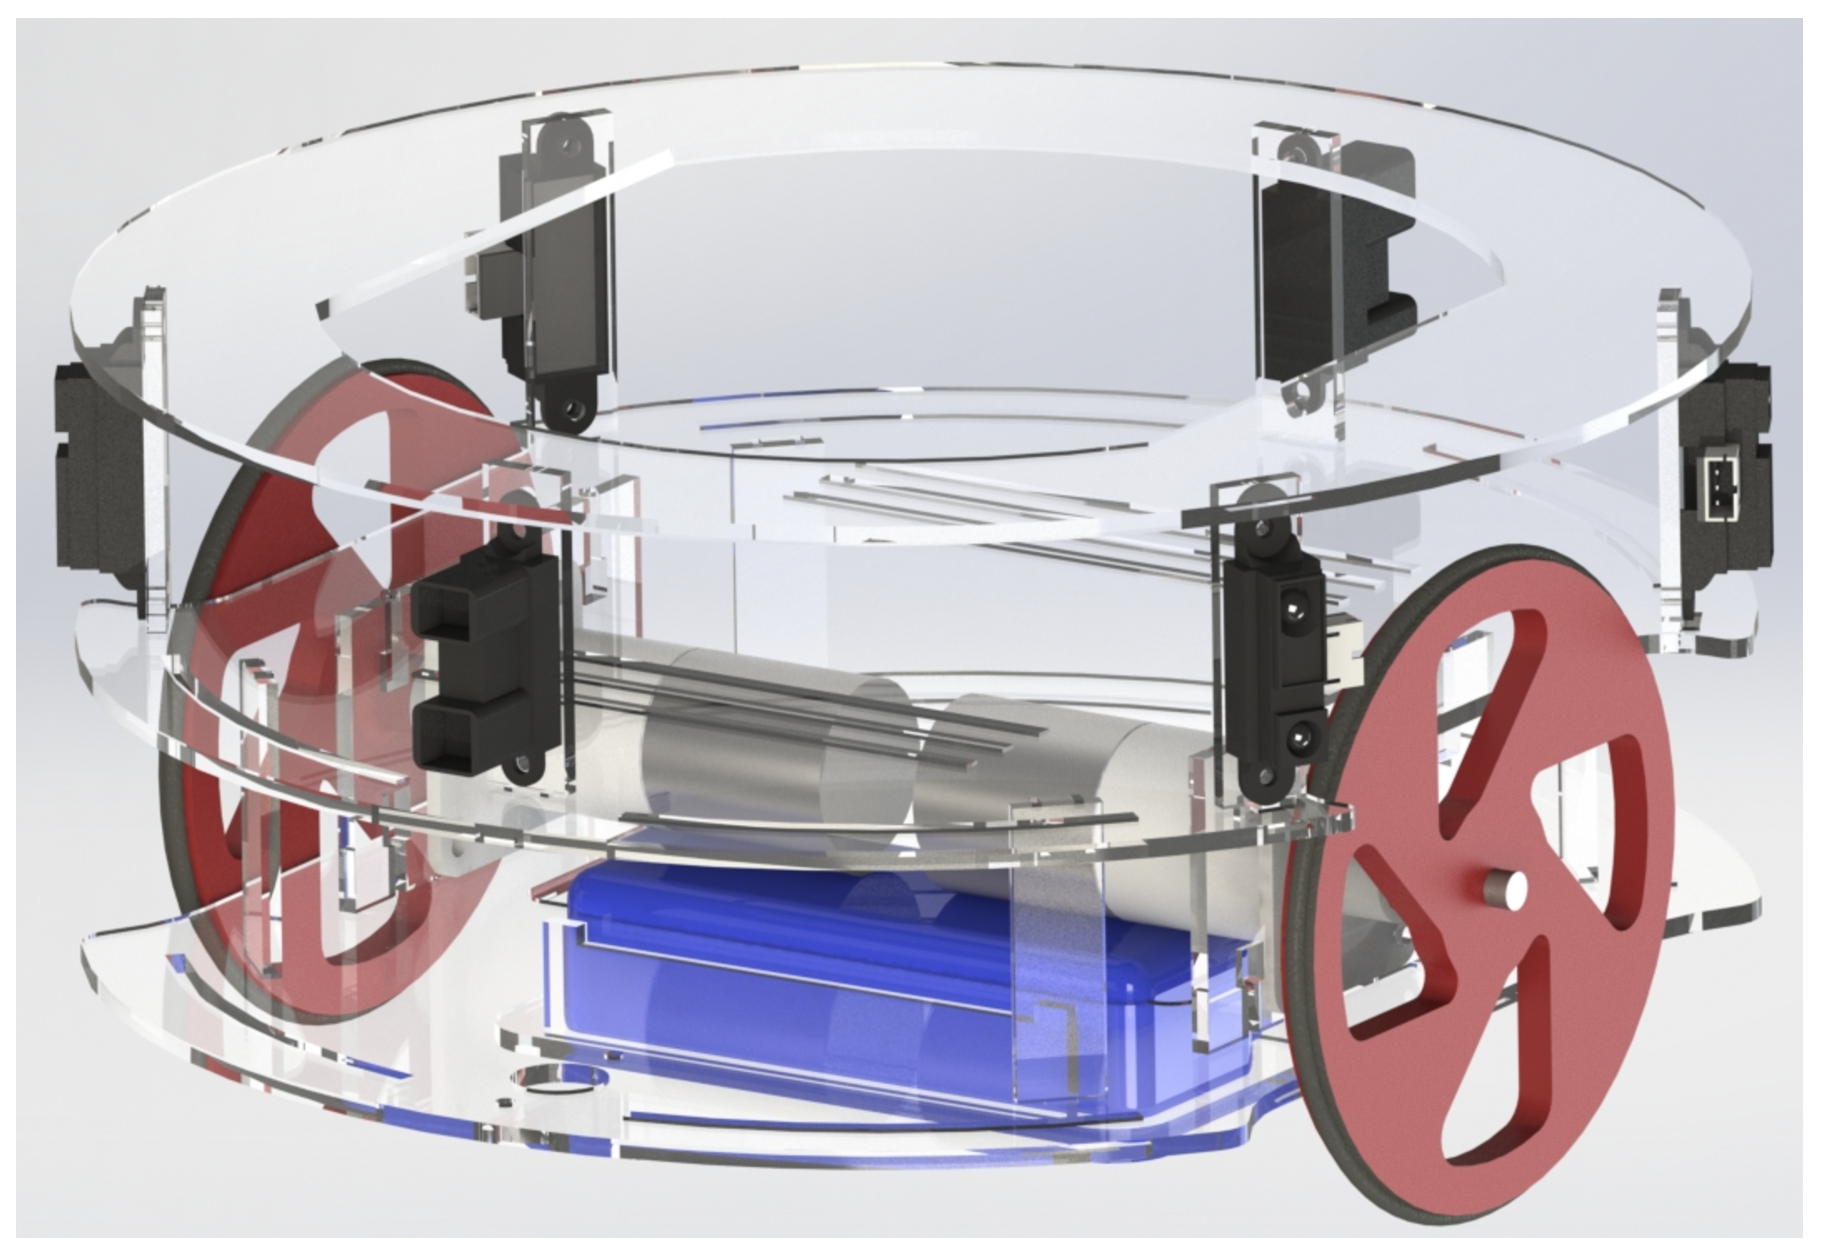
\includegraphics[width=\columnwidth]{render.eps}%
\caption{Esqueleto de la plataforma junto con sus partes mecánicas. Se aprecia la disposición de la batería debajo de los motores, la forma de las ruedas y la distribución equilibrada de los sensores en la perisferia.}%
\label{render}%
\end{figure}

Las ruedas poseen un cuerpo angosto con el fin de ahorrar de material, pero brindando firmeza para poder llevar el peso de la plataforma sin problemas. El diámetro de las ruedas es de $11\mathrm{cm}$, proporcionando una velocidad máxima suficiente para una plataforma experimental. La ruedas están impresas en 3D y se le agregaron anillos de goma para mejorar la adherencia a la superficie.

Uno de los aspectos importantes del diseño es que tiene la posibilidad de agregar módulos sensoriales en forma de pila. Actualmente, la plataforma cuenta con seis sensores infrarrojos, pero el hecho de poder apilar nuevos módulos otorga gran versatilidad al robot.

El módulo sensorial infrarrojo está basado en una estructura hexagonal, con los sensores distribuidos en los $360^\circ$ del robot, para poder evitar choques en todas las direcciones. Si bien no puede cubrirse toda la circunferencia de la Plataforma porque los sensores son direccionales, se distribuyen de forma de optimizar la detección de obstáculos. Para cumplir esta condición, los sensores se ubican siguiendo una estructura hexagonal, colocando los de mayor rango en el frente y en la parte posterior, y completando los costados con los sensores de menor alcance.

Finalmente, cabe destacar que el esqueleto del robot se obtuvo fresando planchas de material mdf de $3\mathrm{mm}$. Ésto nos permite decir que la plataforma es de fácil y rápida reproducción, y por sobre todo, de bajo costo.

\section{Selección del módulo de comunicación inalámbrico}

Para poder recibir todas las instrucciones de control y poder transmitir la información adquirida por los sensores infrarrojos, era de vital importancia que la plataforma contara con un módulo de comunicación inalámbrica. Comercialmente, existen distintos módulos optimizados para aplicaciones basadas en sistemas embebidos que implementan distintos protocolos de comunicación. El objetivo de esta sección es presentar las características de dichos módulos, realizando un análisis comparativo que nos permita escoger el más indicado para nuestra aplicación.

\subsection{Bluetooth}

Bluetooth es un estándar de comunicaciones inalámbricas establecido para conexiones de corto alcance, entre un amplio número de dispositivos. El bajo consumo de potencia es uno de los pilares de este estándar, haciéndolo ideal para implementaciones móviles alimentadas con baterías. El estándar IEEE 802.15.1 presenta una WPAN (Red de Área Personal Inalámbrica, por sus siglas en inglés \textit{Wireless Personal Area Network}) que utiliza tecnología inalámbrica Bluetooth.

La técnica de modulación implementada consiste en la tecnología de espectro espandido, también conocido como acceso múltiple por división de códigos con saltos de frecuencias CDMA-FH, por sus siglas en inglés \textit{Code Division Multiple Access with Frecuency Hopping}. Recordemos que los sistemas de multiplexación permiten la comunicación entre múltiples nodos, a través de un canal común a todos. CDMA emplea una tecnología de espectro expandido y un esquema especial de codificación, por el que a cada transmisor se le asigna un código único, escogido de forma que sea ortogonal respecto al del resto; el receptor capta las señales emitidas por todos los transmisores al mismo tiempo, pero gracias al esquema de codificación puede seleccionar la señal de interés si conoce el código empleado a pesar que todas las señales compartan la misma frecuencia. Además se agregan saltos de frecuencia, que consiste en que un transmisor cambia su frecuencia de trabajo entre todas las disponibles, basándose en un algoritmo planeado previamente o en uno aleatorio. Estas funciones del transmisor se sincronizan con el receptor, de forma que éste sintonice la frecuencia correcta. Estas características de multiplexación y modulación, hacen que la comunicación de Bluetooth sea robusta en ambientes con mucho ruido y a su vez, muy difícil de interceptar por un nodo que no sea el destinatario de nuestro mensaje. Todo esto sumado a un nivel básico de encriptación, basado en la autentificación y en la generación de una clave de acceso de forma
aleatoria en cada dispositivo, permiten definir un nivel elevado de seguridad en las comunicaciones.

Se han definido dos niveles de potencia, uno de $1mW$, que cubre una distancia de 10 metros, y otro de $100mW$ que cubre una distancia de hasta 100 metros. Dicha tecnología es capaz de transmitir voz o datos en tiempo real, con una capacidad máxima por canal de $720Kbps$, aproximadamente. Actúa en la banda de frecuencia de $2,45GHz$, abierta a cualquier sistema de radio de todo el mundo, con rangos que van de los $2,4GHz$ a los $2,5GHz$.

Existen en el mercado diversos módulos que implementan enlaces Bluetooth, entre los que podemos mencionar:

\begin{itemize}
	\item SD Bluetooth Modem-BlueSMIRF Gold
	\item Bluetooth SMD Module - RN-42 (v6.15)
	\item Bluetooth HC-05 Arduino \cite{bluetooth}
	\item SaBLE-x 2.4 GHz Bluetooth Low Energy (BLE) Module
\end{itemize}

\subsection{ZigBee}

Es el nombre de la especificación de un conjunto de protocolos de alto nivel de comunicación inalámbrica de bajo consumo, basada en el estándar IEEE 802.15.4 de redes inalámbricas de área personal (WPAN). Su objetivo son las aplicaciones que requieren comunicaciones seguras con baja tasa de envío de datos y maximización de la vida útil de sus baterías. En principio, el ámbito donde se preve que esta tecnología cobre más fuerza es en domótica debido a su bajo costo, su topología de red en malla y su fácil integración.

ZigBee puede constar de un máximo de 65535 nodos distribuidos en subredes de 255 nodos, lo que la hace versátil e indicado para una gran variedad de aplicaciones. Tiene un consumo de $30 mA$ cuando el dispositivo está transmitiendo y de $3uA$ en reposo. Además, el sistema ZigBee se queda la mayor parte del tiempo dormido, pudiendo pasar al estado activo en menos de $15 ms$. Con velocidades de 20, 40 y $250 Kbps$ y un alcance en el rango de 10 a 75 metros, ZigBee puede funcionar en las bandas de frecuencia ISM (Industrial, Scientific and Medical) de $2,405-2,480 GHz$ (16 canales), $902-928 MHz$ (10 canales) y $868MHz$ (1 canal), aunque la mayoría de fabricantes optan por la primera.

Los dispositivos basados en el estándar IEEE 802.15.4 consumen poca energía debido a que utilizan ciclos de trabajo muy bajos, permaneciendo en modo \textit{sleep} hasta el 99\% del tiempo de implementación. Tienen la capacidad de despertarse rápidamente y conformar una red ad-hoc, siendo los procesos de transmisión y recepción de datos consume gran parte de la energía.

El estándar IEEE802.15.4 es robusto frente a ruidos, ya que implementa la técnica DSSS (\textit{Direct Sequence Spread Spectrum}), también conocida como acceso múltiple por división de código en secuencia directa DS-CDMA, por sus siglas en inglés \textit{Direct-Sequence Code Division Multiple Access}, en la que cada bit de información a transmitirse es modulado con 4 señales portadoras diferentes. La información transmitida ocupa un mayor ancho de banda, y reduce la densidad espectral de potencia. La señal resultante tiene un espectro muy parecido al del ruido, de tal forma que a todos los radiorreceptores les parecerá ruido menos al que va dirigida la señal. Hay diferentes modulaciones Direct Sequence Spread Spectrum (DSSS) que son Binary Phase Shift Keying (BPSK), y Offset Quadrature Phase Shift Keying (O-QPSK).

Con el objetivo de minimizar las colisiones, el estándar IEEE802.15.4 implementa dos técnicas. Por un lado utiliza CSMA/CA (\textit{Carrier Sense Multiple Access-Collision Avoidance}) en la que cada nodo escucha el medio antes de transmitir. Si la energía es mayor de un cierto nivel, el transceptor espera durante un tiempo aleatorio (\textit{back-off time}) e intenta transmitir nuevamente. Por otro lado, tenemos la técnica GTS (\textit{Guaranteed Time Slot}) en el que un coordinador PAN asigna slots a cada nodo (16 time slots posibles). Al comienzo cada nodo envia un GTS request message al coordinador de la PAN, luego el coordinador envía un mensaje con la información del slot asignado.

Con el fin de establecer una clara diferencia entre ZigBee y IEEE 802.15.4, recalcamos que ZigBee es un estándar que define un conjunto de protocolos de comunicación en redes inalámbricas de corto alcance y baja velocidad, desarrollado por ZigBee Alliance (2002), conformado por cientos de empresas. Adoptó el estándar IEEE 802.15.4 para la definición de capas físicas y MAC, dejando a ZigBee la definición de capas de red y de aplicación. Cabe destacar que los dispositivos ZigBee requieren entre el 2\% y el 10\% del hardware respecto a dispositivos Bluetooth o WiFi.

Dentro de los módulos comerciales basados en ZigBee, podemos mencionar los siguientes:

\begin{itemize}
	\item Microchip MRF24J40MA
	\item Jennic JN5148-001
	\item Atmel ZigBit ATZB-24
	\item Digi/Maxstream XB24 \cite{zigbee}
\end{itemize}

\subsection{WiFi}

El estándar WiFi fue desarrollado por WiFi Alliance, una organización comercial formadas por cientos de empresas que certifica qué equipos cumplan con esta norma, la cual define las capas superiores a aquellas definidas en el estándar IEEE 802.11, adoptado por WiFi.

El IEEE 802.11 es un estándar abierto para WLANs en el que se definen las capas física y de enlace. Usa bandas de frecuencias de 2,4 y $5 GHz$ (banda ISM). Los productos comerciales que se pueden encontrar en la actualidad cumplen con normas 802.11b (1999), 802.11g (2003) y 802.11n (2009). La norma IEEE 802.11n permite mayores velocidades de datos, haciendo uso simultáneo de bandas de 2,4 y $5 GHz$.

Mediante WiFi se pueden implementar dos arquitecturas de red. En primer lugar las redes con acceso por Access Point, que conforman el mayor porcentaje de sistemas comunmente utilizados, ofreciendo gran capacidad de conexión, ya que una vez configurada, la red WiFi permite el acceso de múltiples nodos al mismo punto de acceso, sin problemas de gasto ni infraestructura, siempre que compartan la misma capacidad de transmisión de datos que el punto de acceso. Por otro lado, están las redes inalámbricas Ad Hoc (Wireless Ad Hoc Network) en la que cada nodo participa en la difusión de los datos en la red. La determinación de qué nodos retransmiten los datos está dinámicamente basado en su conectividad.

Si bien el estándar WiFi se creó para ser utilizado en redes locales inalámbricas (WLAN), en la actualidad casi la totalidad de aplicaciones lo utilizan como acceso a Internet. Esto nos permite pensar que la plataforma robótica funcionará en un ambiente que tenga una red WiFi con conexión a Internet, lo que puede abrir un abanico inmenso de posibilidades de control de la plataforma. Si se utiliza WiFi como estándar de comunicación inalámbrica, es posible imaginar un escenario en el cual la unidad de control y la plataforma móvil, no se encuentren en el mismo lugar físico, sino que utilicen Internet para establecer el intercambio de información.

Uno de los problemas más graves a los cuales se enfrenta actualmente la tecnología WiFi es la seguridad. Un muy elevado porcentaje de redes son instaladas por administradores de sistemas y redes por su simplicidad de implementación, sin tener en consideración la seguridad y, por lo tanto, convirtiendo sus redes en redes abiertas sin protección de la información que por ellas circulan. Existen varias alternativas para garantizar la seguridad de estas redes. Las más comunes son la utilización de protocolos de seguridad de datos específicos para los protocolos WiFi como el WEP y el WPA que se encargan de autenticación, integridad y confidencialidad, proporcionados por los propios dispositivos inalámbricos. Actualmente existe el protocolo de seguridad llamado WPA2, que es una mejora relativa a WPA, el cual es el mejor protocolo de seguridad para WiFi hasta el momento.

Algunos de los módulos comerciales que actualmente se encuentran en el mercado, son:

\begin{itemize}
	\item ESP8266
	\item RN-XV WiFly
	\item RN-131-PICTAIL
	\item RN 171-y PICtail Plus
\end{itemize}

\subsection{Análisis y selección del módulo}

El las subsecciones anteriores se presentaron las características y ventajas de distintos estándares de comunicación inalámbrica que podrían utilizarse para la aplicación específica que se desarrolla en este trabajo. Para poder elegir cuál de ellas es la más indicada, es conveniente analizar distintos aspectos tanto de los módulos disponibles como de los estándares, relacionados con los requerimientos de la aplicación.

Uno de los aspectos más importantes a tener en cuenta es el consumo de potencia de los módulos. Al estar destinados para aplicaciones inalámbricas, todos los módulos buscan reducir el consumo de potencia, siendo el protocolo ZigBee el más eficiente en este aspecto. Para nuestra aplicación, el consumo es una característica importante ya que afecta la duración de la carga de la batería. Sin embargo, el consumo de los motores es mucho mayor que el de los módulos, por lo que el impacto de éstos sobre la carga de la batería no es primordial.

La plataforma necesita comunicarse con la unidad de control para informar el estado de los sensores y para recibir los comandos relacionados con la velocidad de cada uno de los motores, información que se intercambia cada intervalos regulares de un segundo. Esto pone en evidencia que los requerimientos de velocidad de transmisión no son exigentes, permitiendo establecer que cualquiera de los estándares cumple de forma holgada con la velocidad requerida. Por otro lado, como la plataforma estará destinada para aplicaciones de investigación y desarrollo, no es necesario tener consideraciones especiales sobre la seguridad de la comunicación.

Finalmente, analizando cuestiones económicas, de disponibilidad y de facilidad de conexión con el microcontrolador, se llega a la conclusión que todos los módulos son similares, ya que han sido específicamente diseñados para trabajar en sistemas embebidos. Los módulos incluidos como ejemplos anteriormente, representan costos similares y se encuentran disponibles para su compra por Internet.

Teniendo en cuenta lo expresado anteriormente, se elige el módulo ESP8266. Como se demostró que cualquiera de estos módulos podría ser utilizado para esta aplicación, se elige uno que implementa una red WiFi debido a la capacidad de conexión por Internet. Como se dijo anteriormente, al elegir este protocolo podemos usar el sistema por más que la unidad de control y la plataforma no se encuentren en el mismo espacio físico, siempre y cuando ambos tengan acceso a una red WiFi con conexión a Internet (algo totalmente trivial en nuestro días).

\section{Electrónica del robot}

La circuitería del robot se puede separar en cuatro partes:

\begin{itemize}
	\item Motores y circuito de control de giro.
	\item Sensores infrarrojos.
	\item Módulo de comunicación inalámbrica.
	\item Microcontrolador.
\end{itemize}

En la Fig. \ref{diagrama_bloques} se observa un diagrama que explica la relación entre las distintas partes que integran la plataforma. En esta Sección, se realiza un análisis de cada una de ellas, explicando sintéticamente su diseño y funcionamiento.

\begin{figure*}%
\centering\includegraphics[scale=1]{diagrama_bloques.eps}%
\caption{Diagrama en bloques de la plataforma robótica, donde se distinguen los circuitos montados sobre la plataforma móvil, la unidad de control que se encuentra en la computadora y el enlace inalámbrico entre ambos, a través de comunicación Wi-Fi.}%
\label{diagrama_bloques}%
\end{figure*}

\subsection{Motores y circuito de control de giro}

Los motores elegidos para el proyecto son motores de corriente continua de $12\mathrm{V}$, que alcanzan una velocidad máxima de $50\mathrm{rpm}$ a través de una caja reductora que aumenta el par disponible. Para llevar a cabo el control de los mismos se utiliza un módulo driver de desarrollo, disponible en el mercado. El motivo de esta elección es que este módulo brinda una solución sencilla y económica al problema del control de los motores a través de una señal PWM. El módulo elegido es el doble puente H L298n, el cual se muestra en la Fig. \ref{driver_motores}.

El driver se alimenta con $12 V$ y utiliza esta tensión para alimentar los motores mediante las dos salidas destinadas para este fin. Cuenta con un regulador de $5V$ que provee la tensión necesaria para alimentar el integrado L298N, que es el encargado de definir el sentido de giro de cada motor. El módulo cuenta con dos grupos de tres entradas, un grupo para cada motor. Una de las entradas es un enable \textbf{En} que permite definir si el motor gira o no, dependiendo si se le aplica un ``1'' lógico o un ``0'' lógico; en cambio, si se aplica una señal de PWM en esta entrada, se puede modificar la velocidad del motor. Las entradas \textbf{in1} e \textbf{in2} restantes definen el sentido de giro del motor, dependiendo de la combinación lógica que en ellas se aplique: para ``10'' el motor gira a la derecha, para ``01'' gira a la izquierda y se detiene cuando la combinación es ``00''. Para el caso de ``11'', no se puede predecir el sentido de giro del motor, por lo que esta combinación debe ser evitada.

\begin{figure}[H]%
\centering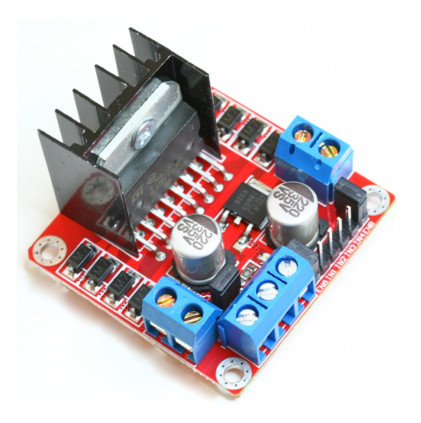
\includegraphics[scale=0.9]{driver_motores.eps}%
\caption{Módulo driver L298N con doble puente H, encargado de controlar el sentido y la velocidad de giro de los motores. Cuenta con dos borneras de dos terminales para la conexión de los motores, con una bornera para la alimentación de la placa y con una tira de pines para las entradas de control.}%
\label{driver_motores}%
\end{figure}

\subsection{Sensores infrarrojos}

Es fundamental para este tipo de sistemas autómatas, tener la capacidad de detectar objetos que puedan interponerse en su trayectoria. Mejor aún si se puede conocer la distancia a la que se encuentra el obstáculo, para tomar diferentes decisiones en base a esta información. Por estas razones, la plataforma cuenta con los sensores infrarrojos medidores de distancia GP2Y0A02YK0F \cite{sensor1} y GP2Y0A21YK0F \cite{sensor2}, los cuales se muestran en la Fig. \ref{sensores}. El primero de ellos tiene un rango de detección de $20\mathrm{cm}$ a $150\mathrm{cm}$; se observan dos de estos dispositivos, uno en la parte frontal y otro en la posterior. Por otro lado, el sensor GP2Y0A21YK0F tiene un alcance de $10\mathrm{cm}$ a $80\mathrm{cm}$, menos preciso que el anterior, por lo que se tiene cuatro de ellos, colocados al costado del robot.

\begin{figure}%
\centering\includegraphics[scale=1]{fotos_sensores.eps}%
\caption{Sensores infrarrojos utilizados en la plataforma. A la izquierda se encuentra el sensor de mayor alcance, cuyo rango es de $20\mathrm{cm}$ a $150\mathrm{cm}$. A la derecha se observa el sensor cuyo rango es de $10\mathrm{cm}$ a $80\mathrm{cm}$}%
\label{sensores}%
\end{figure}

\subsection{Módulo de comunicación inalámbrica}

\begin{figure}%
\centering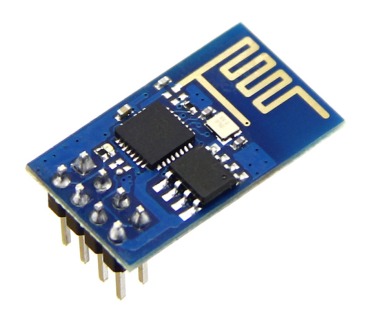
\includegraphics[scale=1]{esp.eps}%
\caption{Módulo comercial de comunicación Wi-Fi ESP8266. Este dispositivo es el encargado de establecer una conexión inalámbrica entre la plataforma móvil y la unidad de control.}%
\label{esp}%
\end{figure}

El ESP8266 es un módulo Serie a Wi-Fi de bajo costo que puede trabajar como servidor en una red Wi-Fi, estableciendo puertos de comunicación que permiten que diversos clientes puedan comunicarse con el módulo, o bien como cliente de otras aplicaciones. Una vez implementada la comunicación entre los distintos nodos de la red, ya sea que la placa funcione como cliente o servidor, se genera un puente bidireccional que permite el intercambio de datos mediante Wi-Fi. Por lo tanto, el módulo ESP8266 permite que cualquier diseño basado en microcontrolador adquiera la capacidad de establecer una comunicación inalámbrica a través de Internet, utilizando una interfaz serie como la UART, que se encuentra disponible en cualquier microcontrolador del mercado.

\subsubsection{Características de la placa}

\begin{itemize}
	\item Protocolo 802.11 b/g/n
	\item Wi-Fi Direct (P2P), soft-AP
	\item TCP/IP protocol stack integrada
	\item T/R RF switch, balun, LNA, amplificador de potencia y red de adaptación integrada
	\item PLL, reguladores, y unidades de manejo de potencia integradas
	\item +19.5dBm de potencia de salida para el modo 802.11b
	\item Sensor de temperatura integrado
	\item Soporta antena diversity
	\item Corriente de fuga de apagado $< 10\mathrm{\mu A}$
	\item CPU de 32 bits integrada de baja potencia, que puede ser usada como el procesador de la aplicación
	\item SDIO 2.0, SPI, UART
	\item A-MPDU y A-MSDU e intervalo de guarda de 0.4s
	\item ``Wake up'' y transmisión de paquetes en menos de 2ms
	\item Consumo menor a 1.0mW en standby (DTIM3)
\end{itemize}

\subsubsection{Conexión de la placa}

Como se explicó anteriormente, la comunicación del módulo con el microprocesador se realiza a través de una UART, por lo que dos de los puertos del microcontrolador se utilizan para este fin. En la Fig. \ref{conexion_wifi} se puede apreciar un esquema de conexión de la placa.

\begin{figure}[H]%
\centering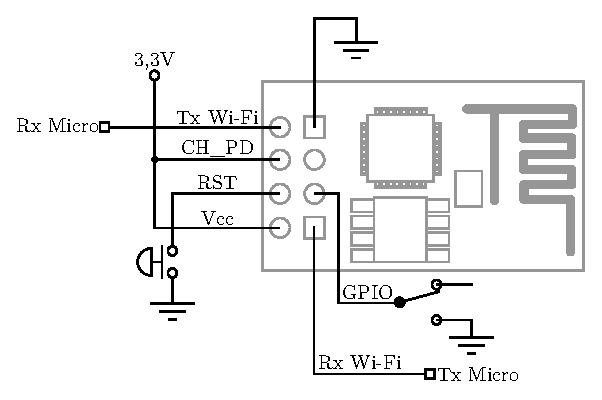
\includegraphics[width=\columnwidth]{conexion_wifi.eps}%
\caption{Esquema de conexión del módulo Wi-Fi.}%
\label{conexion_wifi}%
\end{figure}

Tal como se observa en la Fig. \ref{conexion_wifi}, la alimentación necesaria es de $3,3 V$, la cual se encuentra disponible en pines específicos de nuestro microcontrolador. Por otro lado, el módulo cuenta con una entrada de reset, que lo reinicia cuando se conecta a masa. Es por ello que se incluye un pulsador en este pin para poder resetear el dispositivo de ser necesario.

Otra de las conexiones que debe explicarse es la del pin GPIO. Cuando este pin se encuentre conectado a masa, la placa se encuentra en el modo de actualización de firmware, que le permite al usuario cargar un nuevo archivo de configuración a través del puerto serie. Por lo tanto, es importante recordar que este pin se encuentre desconectado durante el funcionamiento normal de la placa y que sólo se conecte a masa cuando se desee actualizar el firmware del módulo.

\subsubsection{Firmware}

Para que el módulo pueda interpretar los comandos que le envía el microcontrolador a través del puerto serie, es necesario cargarle un archivo de configuración específico. Hay distintas formas de actualizar el firmware de la placa, dependiendo de si se trabaja con Windows o Linux \cite{firmware}. En el primer caso se encuentra disponible una GUI sencilla que permite cargar los archivos de manera interactiva. Por otro lado, en Linux deben seguirse una serie de pasos en la consola. Para este proyecto, se probaron las dos posibilidades, pero finalmente utilizamos la interfaz gráfica provista para Windows, ya que el resto del proyecto se realizó con este sistema operativo.

La placa puede responder a distintos tipos de comandos, siendo comandos AT y LUA los más conocidos y utilizados para este tipo de aplicaciones. Sin embargo, luego de cierta investigación, se descubrió un firmware basado en MicroPython que permite interpretar comandos de Python. MicroPython funciona como una consola que puede ser embebida en un sistema basado en microcontrolador. De esta forma, el módulo puede ser controlado mediante código Python volcado en el puerto serie. Debido a que la clase Socket de Python, que permite establecer puertos de comunicación TCP/IP, se encuentra ampliamente desarrollada, se utiliza este firmware para el desarrollo del proyecto.

Hay ciertas aclaraciones que deben realizarse. En primer lugar, es importante recordar que para cargar el firmware correspondiente en la placa el pin GPIO debe estar conectado a masa, y que debe desconectarse durante el uso normal de la placa. Por otro lado, la velocidad de comunicación serie no es la misma durante la carga del archivo de configuración, que durante el uso del módulo con código Python. En primer lugar la velocidad debe ser establecida en 9600 baudios, mientras que para el uso de la placa la velocidad de comunicación debe ser de 115200 baudios.

\subsubsection{Configuración del puerto inalámbrico}

Una vez que se ha cargado el firmware deseado, y la placa se encuentra correctamente conectada a la alimentación y al puerto serie del microcontrolador, el próximo paso es configurar el puerto de comunicación que será utilizado para transmitir datos entre la plataforma y el control principal que se encuentra en la computadora. Todas las funciones de Python necesarias para este fin, se encuentran dentro de la clase Socket. Aquí, no se hace mención explícita a ninguna de estas funciones, sino que se trata de describir el proceso de forma general.

En primer lugar, es necesario conectar el módulo ESP8266 a una red Wi-Fi. Cuando se establece esta conexión, la red le asigna una dirección de IP al módulo, la cual será utilizada para crear el puerto de comunicación. En este proyecto, el módulo actúa como servidor, es decir que es el encargado de generar el puerto de comunicación y de aceptar o rechazar aquellos potenciales clientes que intenten conectarse a dicho puerto. En síntesis, una vez conectado a la red Wi-Fi y definida la dirección de IP en dicha red, el módulo crea un puerto de comunicación TCP/IP y aguarda a que algún cliente solicite conectarse con la placa; si es el cliente que el módulo estaba esperando, la comunicación es establecida y puede procederse a la transmisión de datos.

\subsection{Microcontrolador}

Para realizar todo el procesamiento de la información adquirida por los sensores, y para controlar el funcionamiento de la Plataforma, se utiliza la placa FRDM-KL46Z \cite{placa_freescale1} de Freescale, que es una plataforma de desarrollo de bajo costo perteneciente a la familia de microcontroladores KL4x de la serie Kinetis L construido con el procesador ARM Cortex-M0+ de 32 bits que funciona a una frecuencia de 48MHz. Dentro de las principales características de esta placa se encuentran un sencillo acceso a las puertos I/O del microcontrolador, built−in debug y operaciones de bajo consumo. En la Fig. \ref{micro} se puede observar la placa utilizada.

\begin{figure}[H]%
\centering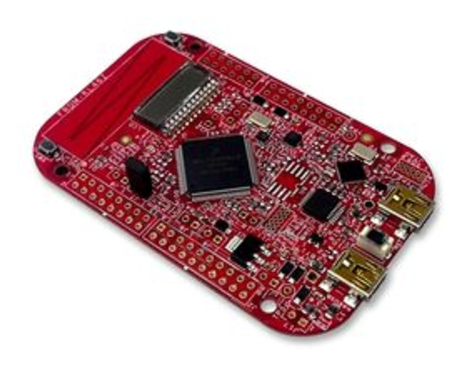
\includegraphics[scale=1]{micro.eps}%
\caption{Placa de desarrollo FRDM-KL46Z de Freescale. Este dispositivo es el encargado de procesar la información provista por los sensores, para luego enviarla a la unidad de control mediante el módulo inalámbrico. Además, establece la velocidad y sentido de giro de los motores.}%
\label{micro}%
\end{figure}

Es importante aclarar que otra de las funciones principales desarrolladas por esta placa es la comunicación con el módulo ESP8266 mediante el puerto serie. El micro es el encargado de recolectar la información de los sensores para luego enviarla, mediante el módulo inalámbrico, a la computadora encargada del control central del sistema. Además, por el mismo medio recibe la indicación de la velocidad que debe desarrollar cada uno de los motores para seguir los comandos ingresados a través del joystick y para evitar el choque con los obstáculos detectados por los sensores infrarrojos.

\section{Software}

El proyecto presentado en este trabajo puede ser dividido en dos partes. Por un lado, está la plataforma móvil compuesta por las distintas partes descriptas en la sección anterior, y por otro lado, se encuentra el software de control principal basado en LabView.

Considerando a la plataforma como una unidad, su tarea es recolectar y enviar al control la información obtenida a través de los sensores infrarrojos, configurar el puerto de comunicación inalámbrica y controlar la velocidad y sentido de giro de los motores, siguiendo las indicaciones provenientes del control. El programa que se encuentra en el microcontrolador es el encargado de configurar el puerto serie para comunicarse con la placa Wi-Fi, configurar las entradas analógicas/digitales para interpretar las lecturas de los sensores y controlar los motores con señales PWM.

El software basado en LabView que se encuentra en la computadora cumple dos funciones. En primer lugar, tiene la finalidad de proveer una interfaz amigable para el usuario, que le permita de forma interactiva controlar el funcionamiento de la plataforma. En esta GUI se incluye una pantalla donde se puede observar las imágenes en tiempo real obtenidas con la cámara IP; ésta podría utilizarse en caso de que la estación de control y la plataforma no se encuentren el mismo espacio físico. Por otro lado, la principal función del control es procesar la información recibida de los sensores infrarrojos, interpretar los comandos introducidos por el usuario a través del joystick y generar, teniendo en cuenta toda esta información recibida, las velocidades de los motores que serán enviadas vía Wi-Fi a la plataforma.

Para transformar las lecturas de los sensores en una velocidad adecuada de los motores se utiliza el algoritmo de campos potenciales. Para que el robot pueda moverse libremente por el entorno esquivando obstáculos, se lo consideró como una carga inmersa en un campo potencial. Es sabido que dos cargas de la misma polaridad experimentan una fuerza de repulsión, inversamente proporcional al cuadrado de la distancia que las separa. Por lo tanto, si se considera que la plataforma y su entorno, están cargados en forma hipotética por cargas de la misma polaridad, puede suponerse que los obstáculos ejercerán una cierta fuerza de repulsión sobre el robot. Este método, denominado comunmente de campos potenciales, le permite al robot girar y avanzar sin colisionar. Para ello, con cada una de las distancias leídas de los sensores infrarrojos, se calcula una fuerza de repulsión artificial, en la dirección del sensor. La información recibida del joystick es considerada como una fuerza de atracción, ya que indica hacia dónde queremos que se desplace la plataforma. Una vez estimadas las fuerzas individuales, se obtiene la
fuerza resultante que moverá al robot.

La fuerza resultante puede interpretarse como un par de fuerzas, una fuerza lateral, aplicada transversalmente al robot que lo hace rotar, y una componente a lo largo de la dirección del movimiento que lo hace avanzar o retroceder.

\section{Conclusiones y trabajo a futuro}

Actualmente, la Plataforma Robótica cuyo diseño fue explicado en este artículo, se encuentra disponible en los laboratorios del C.I.I.I. Dicho prototipo fue implementado con materiales económicos utilizando una fresa para construir la estructura del robot, cumpliendo con los objetivos iniciales de desarrollar un robot económico de fácil reproducción. Por otro lado, el software diseñado facilita la interacción entre el usuario y la plataforma mediante comandos simples de alto nivel.

Durante el desarrollo del proyecto, surgieron varios inconvenientes que demandaron varias horas de trabajo para su solución, principalmente debido a la falta de documentación disponible. Una de las partes que más problemas presentó fue el módulo de comunicación inalámbrica ESP8266, debido a que es relativamente nuevo y la documentación que se encuentra es variada e imprecisa. En este artículo, si bien no se explicó en detalle cuestiones técnicas del módulo por una cuestión de espacio, se intentó detallar los pasos necesarios para su configuración y utilización, con el fin de orientar a futuros usuarios y prevenirlos del desorden que presenta la información que se encuentra en línea.

Una de las mejoras que se podría realizar a este proyecto es la de utilizar la información obtenida con las cámaras como realimentación de la posición de la plataforma dentro del plano de la imagen. De esta forma, se podrían definir trayectorias sin la necesidad de utilizar un joystick. Durante el desarrollo del proyecto, se intentó implementar esta función, pero debido a problemas de comunicación entre las distintas partes y a la falta de tiempo disponible, fue necesario dejar esta característica como trabajo a futuro.

\begin{thebibliography}{4}

\bibitem{encoders} J. Borenstein, H. R. Everett, L. Feng, and D. Wehe, \emph{“Mobile robot positioning-sensors and techniques,”} DTIC Document, Tech. Rep., 1997.

\bibitem{tracking} B. Benfold and I. Reid, \emph{“Stable multi-target tracking in real-time surveillance video”}, in Computer Vision and Pattern Recognition (CVPR), 2011 IEEE Conference on. IEEE, 2011, pp. 34573464.

\bibitem{camara1} T. Krajn k, M. Nitsche, J. Faigl, P. Vanek, M. Saska, L. P. reucil, T. Duckett, and M. Mejail, \emph{“A practical multirobot localization system”,} Journal of Intelligent & Robotic Systems, vol. 76, no. 3-4, pp. 539562, 2014.

\bibitem{camara2} M. Buchheit, A. Allen, T. K. Poon, M. Modonutti,W. Gregson, and V. Di Salvo, \emph{“Integrating different tracking systems in football: multiple camera semi-automatic system, local position measurement and gps technologies”,} Journal of sports sciences, vol. 32, no. 20, pp. 18441857, 2014.

\bibitem{camara3} A. Ibisch, S. Houben, M. Michael, R. Kesten, and F. Schuller, \emph{“Arbitrary object localization and tracking via multiple-camera surveillance system embedded in a parking garage”,} in IST/SPIE Electronic Imaging. International Society for Optics and Photonics, 2015, pp. 94 070G94 070G.

\bibitem{diego} D. Gonzalez Dondo, L. R. Canali, and J. H. Toloza, \emph{“Aplicacion de un filtro de partículas distribuido para el seguimiento de objetivos en el espacio mediante múltiples observaciones angulares”,} en Actas de las VIII Jornadas Argentinas de Robotica 2014.

\bibitem{kulich} M. Kulich, J. Chudoba, K. Kosnar, T. Krajnik, J. Faigl, and L. Preucil, \emph{“Syrotekdistance teaching of mobile robotics”,} Education, IEEE Transactions on, vol. 56, no. 1, pp. 1823, 2013.

\bibitem{sensor1} \emph{Sensor Infrarrojo medidor de distancia, GP2Y0A02YK0F Datasheet}. Sharp

\bibitem{sensor2} \emph{Sensor Infrarrojo medidor de distancia, GP2Y0A21YK0F Datasheet}. Sharp

\bibitem{bluetooth} \url{https://www.rcscomponents.kiev.ua/datasheets/hc_hc-05-user-instructions-bluetooth.pdf}

\bibitem{zigbee} \url{http://www.digi.com/pdf/ds_xbeemultipointmodules.pdf}

\bibitem{wifi} \url{https://www.adafruit.com/datasheets/ESP8266_Specifications_English.pdf}

\bibitem{firmware} \url{https://learn.adafruit.com/building-and-running-micropython-on-the-esp8266?view=all}

\bibitem{placa_freescale1} \emph{FRDM$-$KL46Z User’s Manual}, Freescale Semiconductor Inc., Microcontroller Solutions Group.

\end{thebibliography}

\end{document}


